\documentclass[11pt]{exam}
\RequirePackage{amssymb, amsfonts, amsmath, latexsym, verbatim, xspace, setspace}
\RequirePackage{tikz, pgflibraryplotmarks}

\usepackage[margin=1in]{geometry}

\singlespacing
\usepackage{graphicx}



\begin{document}

% Here's where you edit the Class, Exam, Date, etc.
\newcommand{\name}{Josh Gibbs}
\newcommand{\examnum}{Exam III}
\newcommand{\examdate}{\today}

% These commands set up the running header on the top of the exam pages
\pagestyle{head}
\firstpageheader{}{}{}
\runningheader{\name}{\examnum\ - Page \thepage\ of \numpages}{\examdate}
\runningheadrule






\noindent
\large\textbf{MATH 185 - 88491} \hfill \textbf{Fall 2014} \\
\large\textbf{Exam III} \\
\\
\normalsize Name: \makebox[2in]{\hrulefill} \hfill \textbf{Date:} \makebox[2in]{\hrulefill}\\

You have one week to complete this exam. The solutions to each problem should be written on separate sheets of paper with this sheet stapled to the front. You may use your textbook and course notes but all written work must be your own.
\\\\\\\\\\\\\\\\\\\\
Bill,\\
\indent I know we didn't have to do this assignment in LaTeX, but I've kind of wanted to learn for a while now, so I decided to teach myself. I grossly underestimated the amount of time it would take to write this test in LaTeX. I can't say I ever really look forward to writing anything in this again. And that's all I've really got to say about that. 
\\
\\
All of the source files for this document can be found here:\\
\indent https://github.com/uPaymeiFixit/calculus/tree/master/Exam\%20III










\newpage
1. Sketch the curve defined by each set of parametric equations. Use at least five points in each graph and indicate the direction of each curve. \\
\\
\indent (a) $x = t - t^2,\ y = 3t + 2,\ t \in \Bbb{R} $\\
\newline
\newline
\def\arraystretch{1.5}
\begin{tabular}{ c|c|c }
  $t$ & $x$ & $y$ \\
  \hline
  -2 & -6 & -4 \\
  -1 & -2 & -1 \\
   0 &  0 &  2 \\
   1 &  0 &  5 \\
   2 & -2 &  8 \\
\end{tabular}\\
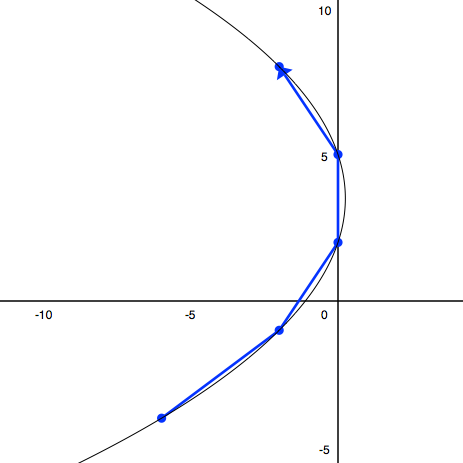
\includegraphics[width=3in]{g1a.png}




\newpage
1. Sketch the curve defined by each set of parametric equations. Use at least five points in each graph and indicate the direction of each curve. \\
\\
\indent (b) $x = -1 + 5\sin t,\ y = 3 + 2 \cos t,\ 0 \leq t \leq 2\pi$\\
\newline
\newline
\def\arraystretch{1.5}
\begin{tabular}{ c|c|c }
  $t$ & $x$ & $y$ \\
  \hline
  0                & -1    & 5 \\
  $\frac{\pi}{3}$  &  3.33 & 4 \\
  $\frac{2\pi}{3}$ &  3.33 & 2 \\
  $\pi$            & -1    & 1 \\
  $\frac{4\pi}{3}$ & -5.33 & 2 \\
  $\frac{5\pi}{3}$ & -5.33 & 4 \\
\end{tabular}\\
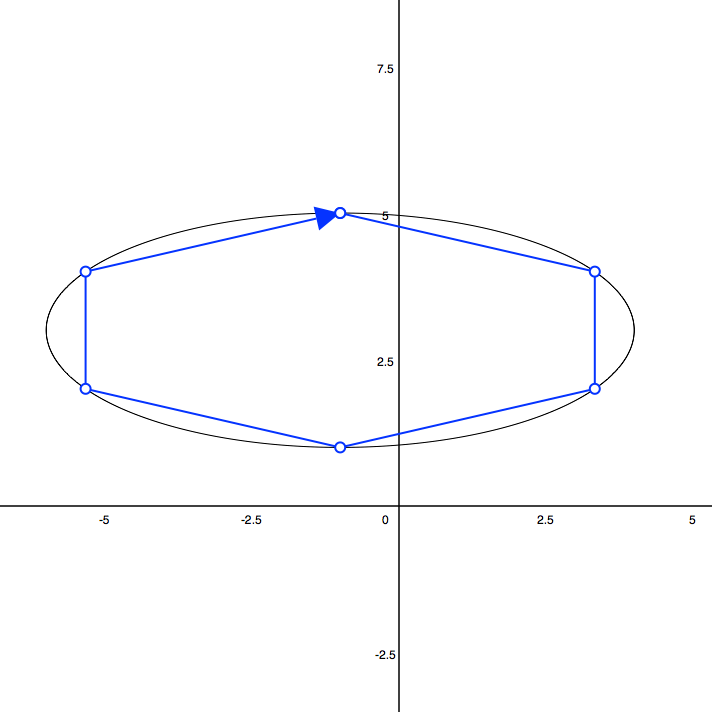
\includegraphics[width=3in]{g1b.png}




\newpage
1. Sketch the curve defined by each set of parametric equations. Use at least five points in each graph and indicate the direction of each curve. \\
\\
\indent (c) $x = e^t - 1,\ y = e^{2t},\ t \in \Bbb{R} $\\
\newline
\newline
\def\arraystretch{1.5}
\begin{tabular}{ c|c|c }
  $t$ & $x$ & $y$ \\
  \hline
  -1   & -0.63 & 0.14 \\
  -0.5 & -0.39 & 0.37 \\
   0   &  0    & 1    \\
   0.5 &  0.65 & 2.72 \\
   1   &  1.72 & 7.39 \\
\end{tabular}\\
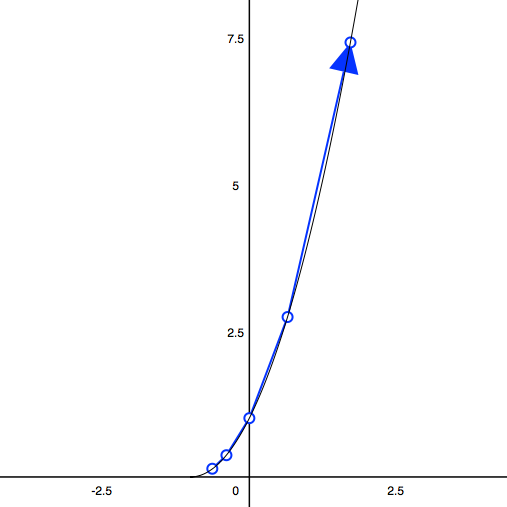
\includegraphics[width=3in]{g1c.png}




\newpage
1. Sketch the curve defined by each set of parametric equations. Use at least five points in each graph and indicate the direction of each curve. \\
\\
\indent (d) $x = 2 - \tan t,\ y = -1 + 2\sec t,\ -\pi/2 < t < \pi/2 $\\
\newline
\newline
\def\arraystretch{1.5}
\begin{tabular}{ c|c|c }
  $t$ & $x$ & $y$ \\
  \hline
  $\frac{-\pi}{3}$ & 3.73 & 3    \\
  $\frac{-\pi}{4}$ & 3    & 1.83 \\
   0               & 2    & 1    \\
  $\frac{\pi}{4}$  & 1    & 1.83 \\
  $\frac{\pi}{3}$  & 0.27 & 3    \\
\end{tabular}\\
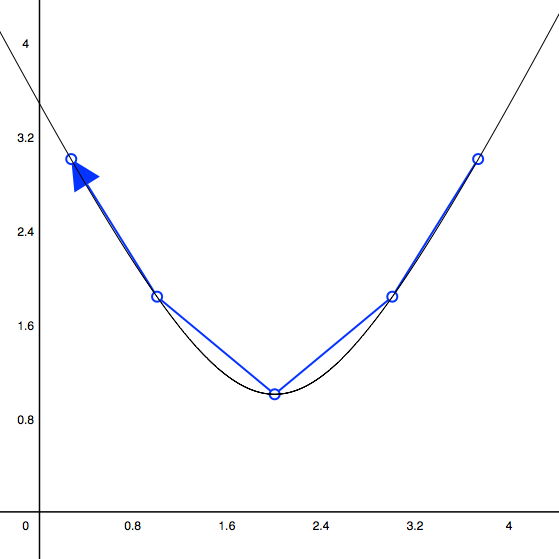
\includegraphics[width=3in]{g1d.png}




\newpage
2. Eliminate the parameter from each of the parametric representations given in problem (1) to find a Cartesian equation for each curve. What types of curves are these? \\
\\
\indent (a) $x = t - t^2,\ y = 3t + 2,\ t \in \Bbb{R} $\\
\newline
\newline
First we find $t$ in terms of $y$.
\begin{eqnarray*}
y&=&3t+2\\
\frac{y-2}{3}&=&t
\end{eqnarray*}
\\
Then we plug $t$ into our $x$ equation.
\begin{eqnarray*}
x&=&t-t^2\\
x&=&\frac{y-2}{3}-\left(\frac{y-2}{3}\right)^2\\
x&=&\frac{y-2}{3}-\frac{y^2-4y+4}{9}\\
x&=&\frac{3(y-2) - (y^2-4y+4)}{9}\\
x&=&\frac{3y-6 - y^2+4y-4}{9}\\
x&=&\frac{-y^2+7y-10}{9}
\end{eqnarray*}

The resulting graph is a parabola opening toward the -x axis.




\newpage
2. Eliminate the parameter from each of the parametric representations given in problem (1) to find a Cartesian equation for each curve. What types of curves are these? \\
\\
\indent (b) $x = -1 + 5\sin t,\ y = 3 + 2 \cos t,\ 0 \leq t \leq 2\pi$\\
\newline
\newline
First we find $\sin t$ and $\cos t$.\\
\\
\noindent\begin{minipage}{.5\linewidth}
\begin{equation*}
  \frac{x+1}{5}=\sin t
\end{equation*}
\end{minipage}%
\begin{minipage}{.5\linewidth}
\begin{equation*}
  \frac{y-3}{2}=cos t
\end{equation*}
\end{minipage}
\\
\\
Then, using the trig identity $\sin^2 t + \cos^2 t = 1$, we find the equation:
$$\left(\frac{x+1}{5}\right)^2 + \left(\frac{y-3}{2}\right)^2 = 1$$

The resulting graph is an ellipse centered at (-1,3).




\newpage
2. Eliminate the parameter from each of the parametric representations given in problem (1) to find a Cartesian equation for each curve. What types of curves are these? \\
\\
\indent (c) $x = e^t - 1,\ y = e^{2t},\ t \in \Bbb{R} $\\
\newline
\newline
First we find $t$ in terms of $x$:\\
\begin{eqnarray*}
e^t &=& x + 1\\
\ln e^t &=& \ln (x+1)\\
t &=& \ln (x+1)\\
\end{eqnarray*}
\\
\\
Then we plug $t$ into our $y$ equation:
$$y = e^{2\ln (x+1)}$$
The resulting graph is an exponential curve (similar to the graph of $y=e^x$).




\newpage
2. Eliminate the parameter from each of the parametric representations given in problem (1) to find a Cartesian equation for each curve. What types of curves are these? \\
\\
\indent (d) $x = 2 - \tan t,\ y = -1 + 2\sec t,\ -\pi/2 < t < \pi/2 $\\
\newline
\newline
First we find $\sec t$ and $\tan t$.\\
\\
\noindent\begin{minipage}{.5\linewidth}
\begin{equation*}
  \frac{y+1}{2}=\sec t
\end{equation*}
\end{minipage}%
\begin{minipage}{.5\linewidth}
\begin{equation*}
  2-x = \tan t
\end{equation*}
\end{minipage}
\\
\\
Then, using the trig identity $\sec^2 t - \tan^2 t = 1$, we find the equation:
$$\left(\frac{y+1}{2}\right)^2 - \left(2-x\right)^2 = 1$$

The resulting graph is a hyperbolic curve opening upwards and downwards. 




\newpage
3. Find parametric equations for the conic section given by each of the following equations. Describe each curve without drawing a graph. \\
\\
\indent (a) $ 25x^2+9y^2-100x+54y-44=0 $\\
\begin{eqnarray*}
25x^2-100x+9y^2+54y &=& 44\\
25(x^2-4x) + 9(y^2+6y) &=& 44\\
25(x^2-4x+4) + 9(y^2+6y+9) &=& 44+100+81\\
25(x-2)^2 + 9(y+3)^2 &=& 225\\
\frac{25(x-2)^2}{225}+\frac{9(y+3)^2}{225}&=&1\\
\frac{(x-2)^2}{9}+\frac{(y+3)^2}{25}&=&1\\
\end{eqnarray*}
The resulting graph is an ellipse centered at (2,-3).\\
\\
Using the trig identity $\sin^2 \theta + \cos^2 \theta = 1$, we can say:\\
\\
\noindent\begin{minipage}{.5\linewidth}
\begin{eqnarray*}
  \frac{(x-2)^2}{9}&=&\cos^2 \theta\\
  \frac{x-2}{3}&=&\cos \theta\\
  x-2 &=& 3\cos \theta\\
  x &=& 3\cos \theta + 2\\
\end{eqnarray*}
\end{minipage}%
\begin{minipage}{.5\linewidth}
\begin{eqnarray*}
  \frac{(y+3)^2}{25}&=&\sin^2 \theta\\
  \frac{y+3}{5}&=&\sin \theta\\
  y+3 &=& 5\sin \theta\\
  y &=& 5\sin \theta -3\\
\end{eqnarray*}
\end{minipage}




\newpage
3. Find parametric equations for the conic section given by each of the following equations. Describe each curve without drawing a graph. \\
\\
\indent (b) $x^2-8x+y^2-12y+51=0$\\
\begin{eqnarray*}
(x^2-8x)+(y^2-12y)&=&-51\\
(x^2-8x+16)+(y^2-12y+36)&=&-51+16+36\\
(x-4)^2+(y-6)^2&=&1\\
\end{eqnarray*}
The resulting graph is a circle with a radius of 1 centered at (4,6).\\
\\
Using the trig identity $\sin^2 \theta + \cos^2 \theta = 1$, we can say:\\
\\
\noindent\begin{minipage}{.5\linewidth}
\begin{eqnarray*}
  (x-4)^2&=&\cos^2 \theta\\
  x-4&=&\cos \theta\\
  x&=&\cos \theta +4\\
\end{eqnarray*}
\end{minipage}%
\begin{minipage}{.5\linewidth}
\begin{eqnarray*}
  (y-6)^2&=&\sin^2 \theta\\
  y-6&=&\sin \theta\\
  y&=&\sin \theta\ +6\
\end{eqnarray*}
\end{minipage}




\newpage
3. Find parametric equations for the conic section given by each of the following equations. Describe each curve without drawing a graph. \\
\\
\indent (c) $16y^2-9x^2-36x+128y+76=0$\\
\begin{eqnarray*}
(16y^2+128y)+(-9x^2-36x)&=&-76\\
16(y^2+8y)-9(x^2+4x)&=&-76\\
16(y^2+8y+16)-9(x^2+4x+4)&=&-76+16*16-9*4\\
16(y+4)^2-9(x+2)^2&=&144\\
\frac{16(y+4)^2}{144}+\frac{-9(x+2)^2}{144}&=&1\\
\frac{(y+4)^2}{9}-\frac{(x+2)^2}{16}&=&1\\
\end{eqnarray*}
The resulting graph is a hyperbola centered at (-2,-4).\\
\\
Using the trig identity $\sec^2 \theta - \tan^2 \theta = 1$, we can say:\\
\\
\noindent\begin{minipage}{.5\linewidth}
\begin{eqnarray*}
  \frac{(y+4)^2}{9}&=&\sec^2 \theta\\
  y+4&=&3\sec \theta\\
  y&=&3\sec \theta -4\\
\end{eqnarray*}
\end{minipage}%
\begin{minipage}{.5\linewidth}
\begin{eqnarray*}
  \frac{(x+2)^2}{16}&=&\tan^2 \theta\\
  x+2&=&4\tan \theta\\
  x&=&4\tan \theta\ -2\
\end{eqnarray*}
\end{minipage}




\newpage
4. Find the length of each of the following curves. \\
\\
\indent (a) The curve given by $x=2t^2,\ y=2t^3$ over $0 \leq t \leq 2$\\
\\
The formula for arc length of a parametric curve is
$$L = \int_a^b \! \sqrt{\left(\frac{\mathrm{d}x}{\mathrm{d}\theta}\right)^2+\left(\frac{\mathrm{d}y}{\mathrm{d}\theta}\right)^2} \, \mathrm{d}\theta$$
So the first step is to find $\frac{\mathrm{d}x}{\mathrm{d}\theta}$ and $\frac{\mathrm{d}y}{\mathrm{d}\theta}$.\\
\noindent
\begin{minipage}{.5\linewidth}
	\begin{eqnarray*}
		x &=& 2t^2\\
 		\frac{\mathrm{d}x}{\mathrm{d}\theta}&=&4t\\
	\end{eqnarray*}
\end{minipage}
\begin{minipage}{.5\linewidth}
	\begin{eqnarray*}
  		y&=&2t^3\\
  		\frac{\mathrm{d}y}{\mathrm{d}\theta}&=&6t^2\\
	\end{eqnarray*}
\end{minipage}
Now we plug this in to our formula and solve.\\
\begin{eqnarray*}
	L &=& \int_0^2 \! \sqrt{(4t)^2+(6t^2)^2} \, \mathrm{d}t\\
	L &=& \int_0^2 \! \sqrt{16t^2+36t^4} \, \mathrm{d}t\\
	L &=& \int_0^2 \! \sqrt{(4t^2)(4+9t^2)} \, \mathrm{d}t\\
	L &=& 2\int_0^2 \! t\sqrt{4+9t^2} \, \mathrm{d}t
\end{eqnarray*} 
We will need to use u-substitution to solve this integral.\\
\noindent
\begin{minipage}{.5\linewidth}
	\begin{eqnarray*}
 		L &=& 2\int_0^2 \! t\sqrt{u}\frac{\mathrm{d}u}{18t} \\
 		L &=& \frac{2}{18}\int_0^2 \! \sqrt{u}\ \mathrm{d}u \\
 		L &=& \frac{1}{9}\left[\frac{2u^{3/2}}{3}\right]_0^2 \\
 		L &=& \frac{1}{9}\left[\frac{2(4+9t^2)^{3/2}}{3}\right]_0^2 \\
 		L &=& \frac{1}{9}\left[\frac{2(4+9(2)^2)^{3/2}}{3}-\frac{2(4+9(0)^2)^{3/2}}{3}\right] \\
 		L &=& \frac{1}{9}\left[\frac{2(40)^{3/2}}{3}-\frac{2(4)^{3/2}}{3}\right] \\
 		L &=& \frac{2}{27}\left[(40)^{3/2}-8\right] = \frac{16}{27}\left[10\sqrt{10}-1\right]\\
	\end{eqnarray*}
\end{minipage}
\begin{minipage}{.5\linewidth}
	\begin{eqnarray*}
	  	u &=& 4 + 9t^2\\
  		\mathrm{d}u &=& 18t \mathrm{d}t\\
  		\mathrm{d}t &=& \frac{\mathrm{d}u}{18t}\\\\\\\\\\\\\\\\\\\\\\
	\end{eqnarray*}
\end{minipage}




\newpage
4. Find the length of each of the following curves. \\
\\
\indent (b) The curve given by $x=\cos^3 t,\ y = \sin^3 t$ over $0 \leq t \leq \pi/2\\$
\\
The formula for arc length of a parametric curve is
$$L = \int_a^b \! \sqrt{\left(\frac{\mathrm{d}x}{\mathrm{d}\theta}\right)^2+\left(\frac{\mathrm{d}y}{\mathrm{d}\theta}\right)^2} \, \mathrm{d}\theta$$
So the first step is to find $\frac{\mathrm{d}x}{\mathrm{d}\theta}$ and $\frac{\mathrm{d}y}{\mathrm{d}\theta}$.\\
\noindent
\begin{minipage}{.5\linewidth}
	\begin{eqnarray*}
		x &=& \cos^3 t\\
 		\frac{\mathrm{d}x}{\mathrm{d}\theta}&=&3\cos^2 t (-\sin t)\\
	\end{eqnarray*}
\end{minipage}
\begin{minipage}{.5\linewidth}
	\begin{eqnarray*}
  		y&=&\sin^3 t\\
  		\frac{\mathrm{d}y}{\mathrm{d}\theta}&=&3\sin^2 t \cos t\\
	\end{eqnarray*}
\end{minipage}
Now we plug this in to our formula and solve.\\
\begin{eqnarray*}
	L &=& \int_0^{\pi/2} \! \sqrt{(3\cos^2 t (-\sin t))^2+(3\sin^2 t \cos t)^2} \, \mathrm{d}t\\
	L &=& \int_0^{\pi/2} \! \sqrt{(9\cos^4 t\sin^2 t)+(9\sin^4 t\cos^2 t)} \, \mathrm{d}t\\
	L &=& \int_0^{\pi/2} \! \sqrt{(9\cos^2 t\sin^2 t)(\sin^2 t+\cos^2 t)} \, \mathrm{d}t\\
	L &=& 3\int_0^{\pi/2} \! \cos t \sin t \, \mathrm{d}t\\	
\end{eqnarray*} 
We will need to use integration by parts to solve this integral.\\
\noindent
\begin{minipage}{.5\linewidth}
	\begin{eqnarray*}
 		\int \sin t \cos t &=& \sin^2 t - \int \sin t \cos t \\
 		2\int \sin t \cos t &=& \sin^2 t \\
 		\int \sin t \cos t &=& \frac{\sin^2 t}{2} \\
	\end{eqnarray*}
\end{minipage}
\begin{minipage}{.5\linewidth}
	\begin{eqnarray*}
	  	\int u \, \mathrm{d}v = uv - \int v \, \mathrm{d}u\\
	  	u = \sin t\\
	  	dv = \cos t\\
	  	du = \cos t\\
	  	v = \sin t\\
	\end{eqnarray*}
\end{minipage}
Now that we found the integral, we can plug it back in. 
\begin{eqnarray*}
	L &=& 3\left[\frac{\sin^2 t}{2}\right]_0^{\pi/2} \\
	L &=& 3\left[\frac{\sin^2 \pi/2}{2} - \frac{\sin^2 0}{2}\right] \\
	L &=& \frac{3}{2} \\	
\end{eqnarray*}




\newpage
5. A curve C is defined by the parametric equations $x=t^2,\ y=t^3-3t$. \\
\\
\indent (a) Find equations for the two tangent lines to C at the point (3,0)
\\
The first thing we need to do is find a value for $t$ that satisfies $x=3$ and $y=0$.\\
\noindent
\begin{minipage}{.5\linewidth}
	\begin{eqnarray*}
		x = t^2 &=& 3\\
		t &=& \pm \sqrt{3}\\
	\end{eqnarray*}
\end{minipage}
\begin{minipage}{.5\linewidth}
	\begin{eqnarray*}
  		y = t^3-3t &=& 0\\
  		t &=& 0,\ \pm \sqrt{3}\\  		
	\end{eqnarray*}
\end{minipage}
Since $\pm \sqrt{3}$ are the only values that satisfy both $x$ and $y$, we will only use those.\\
The formula for the slope of a tangent line to a parametric curve is
$$\frac{\mathrm{d}y}{\mathrm{d}x}$$
So now we need to find $\mathrm{d}y$ and $\mathrm{d}x$.\\
\noindent
\begin{minipage}{.5\linewidth}
	\begin{eqnarray*}
		\mathrm{d}y &=& 3t^2 - 3\\
	\end{eqnarray*}
\end{minipage}
\begin{minipage}{.5\linewidth}
	\begin{eqnarray*}
  		\mathrm{d}x &=& 2t\\ 		
	\end{eqnarray*}
\end{minipage}
\begin{eqnarray*}
	\frac{\mathrm{d}y}{\mathrm{d}x} &=& \frac{3t^2 - 3}{2t}\\
	\frac{\mathrm{d}y}{\mathrm{d}x} &=& \frac{3}{2}\left(t-\frac{1}{t}\right)\\
\end{eqnarray*}
Now we can plug in $t = \pm \sqrt{3}$ to find our slope.\\
\noindent
\begin{minipage}{.5\linewidth}
	\begin{eqnarray*}
		\frac{3}{2}\left(( \sqrt{3} )-\frac{1}{( \sqrt{3} )}\right) \\
		\frac{3 \sqrt{3} }{2}\left( \frac{\sqrt{3} }{ \sqrt{3} } -\frac{1}{ \sqrt{3} \sqrt{3} }\right) \\
		\frac{3 \sqrt{3} }{2}\left( 1 -\frac{1}{ 3 }\right) \\
		\frac{3 \sqrt{3} }{2}\left( \frac{2}{ 3 }\right) \\
		\sqrt{3}\\
	\end{eqnarray*}
\end{minipage}
\begin{minipage}{.5\linewidth}
	\begin{eqnarray*}
  		\frac{3}{2}\left(( -\sqrt{3} )-\frac{1}{( -\sqrt{3} )}\right) \\ 
  		\frac{3 \sqrt{3} }{2}\left( \frac{ -\sqrt{3} }{ \sqrt{3} } -\frac{1}{( -\sqrt{3}) (\sqrt{3} )}\right) \\
  		\frac{3 \sqrt{3} }{2}\left( -1 +\frac{1}{3} \right) \\
  		\frac{3 \sqrt{3} }{2}\left( -\frac{2}{3} \right) \\
  		-\sqrt{3}\\
	\end{eqnarray*}
\end{minipage}



\noindent Now we can use point slope form to find our two equations.\\
\noindent
\begin{minipage}{.5\linewidth}
	\begin{eqnarray*}
		y - y_0 &=& m(x-x_0) \\
		y - 0 &=& \sqrt{3}(x-3) \\
		y &=& x\sqrt{3}-3\sqrt{3} \\
	\end{eqnarray*}
\end{minipage}
\begin{minipage}{.5\linewidth}
	\begin{eqnarray*}
		y - y_0 &=& m(x-x_0) \\
		y - 0 &=& -\sqrt{3}(x-3) \\
		y &=& -x\sqrt{3}+3\sqrt{3} \\
	\end{eqnarray*}
\end{minipage}




\newpage
5. A curve C is defined by the parametric equations $x=t^2,\ y=t^3-3t$. \\
\\
\indent (b) Find the points on C where the tangent lines are horizontal or vertical.
\\\\
From the previous question we found that the slope of the tangent line at a certain value of $t$ is:\\
$$\frac{3}{2}\left(t-\frac{1}{t}\right)$$
We know that the slope of a horizontal line is 0, and the slope of a vertical line is $\infty$ (or undefined).\\
Knowing this, we can set our slope to 0 and $\infty$ to find our horizontal and vertical points.\\
\noindent
\begin{minipage}{.5\linewidth}
	\begin{eqnarray*}
		\frac{3}{2}\left(t-\frac{1}{t}\right) &=& 0 \\
		t - \frac{1}{t} &=& 0 \\
		t^2 - 1 &=& 0 \\
		t^2 &=& 1 \\
		t &=& \pm 1 \\
	\end{eqnarray*}
\end{minipage}
\begin{minipage}{.5\linewidth}
	\begin{eqnarray*}
		\frac{3}{2}\left(t-\frac{1}{t}\right) &=& \infty \\
		t &=& 0
	\end{eqnarray*}
\end{minipage}
Now we plug those values for $t$ into our original equation to get points.\\
\noindent
\begin{minipage}{.5\linewidth}
	\begin{eqnarray*}	
		x &=& (1)^2 = 1 \\
		x &=& (-1)^2 = 1 \\
		y &=& (1)^3 - 3(1) = -2\\
		y &=& (-1)^3 - 3(-1) = 2\\
	\end{eqnarray*}
\end{minipage}
\begin{minipage}{.5\linewidth}
	\begin{eqnarray*}
		x &=& (0)^2 = 0 \\
		y &=& (0)^3-3(0) = 0 \\
	\end{eqnarray*}
\end{minipage}
\noindent
\begin{minipage}{.5\linewidth}
	\begin{eqnarray*}
		\mathrm{Horizontal:}\\
		(1,-2),\ (1,2)
	\end{eqnarray*}
\end{minipage}
\begin{minipage}{.5\linewidth}
	\begin{eqnarray*}
		\mathrm{Vertical:}\\
		(0,0)\\
	\end{eqnarray*}
\end{minipage}



\newpage
6. Find the surface area of the solid obtained by rotating the curve given by $x = e^t \cos t,\ y = e^t \sin t$ for $0 \leq t \leq \pi/2$ about the x-axis. \\
\\
The formula for the surface area of a parametric curve is
$$S = \int_\alpha^\beta \! 2\pi y \sqrt{\left(\frac{\mathrm{d}x}{\mathrm{d}t}\right)^2+\left(\frac{\mathrm{d}y}{\mathrm{d}t}\right)^2} \, \mathrm{d}t$$
So the first step is to find $\frac{\mathrm{d}x}{\mathrm{d}t}$ and $\frac{\mathrm{d}y}{\mathrm{d}t}$.\\
\noindent
\begin{minipage}{.5\linewidth}
	\begin{eqnarray*}
		x &=& e^t \cos t\\
 		\frac{\mathrm{d}x}{\mathrm{d}t}&=&e^t (\cos t - \sin t) \\
	\end{eqnarray*}
\end{minipage}
\begin{minipage}{.5\linewidth}
	\begin{eqnarray*}
  		y&=&e^t \sin t\\
  		\frac{\mathrm{d}y}{\mathrm{d}t}&=&e^t (\cos t + \sin t) \\
	\end{eqnarray*}
\end{minipage}
Now we plug this in to our formula and solve.\\
\begin{eqnarray*}
	S &=& \int_0^{\pi/2} \! 2\pi e^t \sin t \sqrt{\left(e^t (\cos t - \sin t)\right)^2+\left(e^t (\cos t + \sin t)\right)^2} \, \mathrm{d}t \\	
	S &=& \int_0^{\pi/2} \! 2\pi e^t \sin t \sqrt{e^{2t}(\cos^2t -\sin t\cos t -\sin t\cos t+\sin^2 t + \cos^2 t+\sin t\cos t+\sin t\cos t+\sin^2 t)} \, \mathrm{d}t \\
	S &=& \int_0^{\pi/2} \! 2\pi e^t \sin t \sqrt{e^{2t}2(\cos^2 t + \sin^2 t)} \, \mathrm{d}t \\	
	S &=& \int_0^{\pi/2} \! 2\pi e^{2t} \sin t \sqrt{2} \, \mathrm{d}t \\
	S &=& 2\pi\sqrt{2} \int_0^{\pi/2} \! e^{2t} \sin t  \, \mathrm{d}t \\	
\end{eqnarray*} 
We will need to use integration by parts to solve this integral.\\
\noindent
\begin{minipage}{.5\linewidth}
	\begin{eqnarray*}
 		\int e^{2t} \sin t &=& e^{2t}(-\cos t) - \int -\cos t \, 2e^{2t} \\
 		\int e^{2t} \sin t &=& e^{2t}(-\cos t) +2 \int \cos t \, e^{2t} \\
	\end{eqnarray*}
\end{minipage}
\begin{minipage}{.5\linewidth}
	\begin{eqnarray*}
	  	\int u \, \mathrm{d}v = uv - \int v \, \mathrm{d}u\\
	  	u = e^{2t} \\
	  	dv = \sin t \\
	  	du = 2e^{2t} \\
	  	v = -\cos t \\
	\end{eqnarray*}
\end{minipage}
Yet again, we will need to use integration by parts to solve this integral.\\\\
\indent[CONTINUED ON NEXT PAGE]\\
\noindent
\begin{minipage}{.5\linewidth}
	\begin{eqnarray*}
 		\int e^{2t} \cos t &=& e^{2t}\sin t - \int \sin t \, 2e^{2t} \\
 		\int e^{2t} \cos t &=& e^{2t}\sin t - 2\int \sin t \, e^{2t} \\
	\end{eqnarray*}
\end{minipage}
\begin{minipage}{.5\linewidth}
	\begin{eqnarray*}
	  	\int u \, \mathrm{d}v = uv - \int v \, \mathrm{d}u\\
	  	u = e^{2t} \\
	  	dv = \cos t \\
	  	du = 2e^{2t} \\
	  	v = \sin t \\
	\end{eqnarray*}
\end{minipage}
Now that we found the integral, we can plug it back into our last integration by parts equation. 
\begin{eqnarray*}
	\int e^{2t} \sin t &=& e^{2t}(-\cos t) +2(e^{2t}\sin t - 2\int \sin t \, e^{2t}) \\
	\int e^{2t} \sin t &=& e^{2t}(-\cos t) +2e^{2t}\sin t - 4\int \sin t \, e^{2t} \\
	5\int e^{2t} \sin t &=& e^{2t}(-\cos t) +2e^{2t}\sin t \\
	\int e^{2t} \sin t &=& \frac{e^{2t}(-\cos t) +2e^{2t}\sin t}{5} \\
	\int e^{2t} \sin t &=& \frac{e^{2t}(2\sin t-\cos t)}{5} \\
\end{eqnarray*}
Now that we found the integral, we can plug it back into our original equation.
\begin{eqnarray*}
	S &=& 2\pi\sqrt{2} \left[\frac{e^{2t}(2\sin t-\cos t)}{5}\right]_0^{\pi/2} \\	
	S &=& 2\pi\sqrt{2} \left[\frac{e^{2(\pi/2)}(2\sin (\pi/2)-\cos (\pi/2))}{5}-\frac{e^{2(0)}(2\sin (0)-\cos (0))}{5}\right] \\
	S &=& 2\pi\sqrt{2} \left[\frac{e^{\pi}(2(1)-(0))}{5}-\frac{{e^0}(2(0)-(1))}{5}\right] \\	
	S &=& 2\pi\sqrt{2} \left[\frac{2e^{\pi}}{5}-\frac{-1}{5}\right] \\
	S &=& 2\pi\sqrt{2} \left[\frac{2e^{\pi}}{5}+\frac{1}{5}\right] \\	
	S &=& 2\pi\sqrt{2} \left[\frac{2e^{\pi}}{5}+\frac{1}{5}\right] \\	
	S &=& \frac{4\pi\sqrt{2}e^\pi}{5} + \frac{2\sqrt{2}\pi}{5} \\
	S &=& \frac{2\pi\sqrt{2}(2e^\pi+1)}{5} \\	
\end{eqnarray*}




\newpage
7. Show that the area of the circle given by $x=r\sin t,\ y=r\cos t,\ 0\leq t\leq 2\pi$, is $A = \pi r^2$. \\
\\
The formula for the area of a parametric curve is
$$A = \int_\alpha^\beta \! g(t) f'(t) \, \mathrm{d}t$$
where $g(t) = y$ and $f(t) = x$.\\\\
So the first step is to find $\frac{\mathrm{d}x}{\mathrm{d}t}$.
\begin{eqnarray*}
  	x&=&r\sin t \\
  	\frac{\mathrm{d}y}{\mathrm{d}t}&=& r\cos t \\
\end{eqnarray*}
Now we plug this in to our formula and solve.\\
\begin{eqnarray*}
	A &=& \int_0^{2\pi} \! r\cos t(r\cos t) \, \mathrm{d}t \\
	A &=& \int_0^{2\pi} \! r^2\cos^2 t \, \mathrm{d}t \\
	A &=& r^2 \int_0^{2\pi} \! \cos^2 t \, \mathrm{d}t \\
\end{eqnarray*} 
Using the trig identity $\cos^2 t = \frac{1+\cos {2t}}{2}$ we can simplify our integral: \\
\begin{eqnarray*}
	A &=& r^2 \int_0^{2\pi} \! \frac{1+\cos {2t}}{2} \, \mathrm{d}t \\
	A &=& r^2 \frac{1}{2} \int_0^{2\pi} \! 1+\cos {2t} \, \mathrm{d}t \\
	A &=& r^2 \frac{1}{2} \left(\int_0^{2\pi} \! 1 \, \mathrm{d}t + \int_0^{2\pi} \! \cos {2t} \, \mathrm{d}t \right) \\
	A &=& r^2 \frac{1}{2} \left(2\pi + \int_0^{2\pi} \! \cos {2t} \, \mathrm{d}t \right) \\
\end{eqnarray*}
We will need to use u-substitution to solve this integral.\\\\
\indent[CONTINUED ON NEXT PAGE]\\
\noindent
\begin{minipage}{.5\linewidth}
	\begin{eqnarray*}
		 A &=& r^2 \frac{1}{2} \left(2\pi + \int_0^{2\pi} \! \cos {u} \, \frac{\mathrm{d}u}{2} \right) \\
		 A &=& r^2 \frac{1}{2} \left(2\pi + \frac{1}{2} \int_0^{2\pi} \! \cos {u} \, \mathrm{d}u \right) \\
		 A &=& r^2 \frac{1}{2} \left(2\pi + \frac{1}{2} [\sin {2t}]_0^{2\pi} \right) \\
		 A &=& r^2 \frac{1}{2} \left(2\pi + \frac{1}{2} (0) \right) \\
		 A &=& \pi r^2 \\
	\end{eqnarray*}
\end{minipage}
\begin{minipage}{.5\linewidth}
	\begin{eqnarray*}
	  	u = 2t \\
	  	du = 2 dt t\\
	  	dt = \frac{du}{2} \\
	\end{eqnarray*}
\end{minipage}


\newpage
8. For each of the given Cartesian equations, find the polar form. For each polar equation, find the Cartesian form. \\
\\
\indent (a) $4y^2 = x$
\\
\begin{eqnarray*}
	4y^2 &=& x \\
	4(r \sin \theta)^2 &=& r\cos \theta \\
	r &=& \frac{4 r^2 sin^2 \theta}{\cos \theta} \\
	\frac{1}{r} &=& \frac{4 \sin^2 \theta}{\cos \theta} \\
	r &=& \frac{\cos \theta}{4 \sin^2 \theta} \\
	r &=& \frac{1}{4}\cot \theta \csc \theta \\
\end{eqnarray*}
\\
\\
\\
\indent (b) $r = 4\sec \theta$
\\
\noindent
\begin{minipage}{.5\linewidth}
	\begin{eqnarray*}
		x &=& 4\sec\theta\cos\theta \\
		x &=& 4 \\
	\end{eqnarray*}
\end{minipage}
\begin{minipage}{.5\linewidth}
	\begin{eqnarray*}
		y &=& 4\sec\theta\sin\theta \\
		y &=& 4\tan\theta \\
	\end{eqnarray*}
\end{minipage}
\\
\\
\indent (c) $xy = 4$
\\
\begin{eqnarray*}
	r\cos\theta r\sin\theta = 4 \\
	r = \frac{2}{\sqrt{\cos\theta\sin\theta}} \\
\end{eqnarray*}
\\
\indent (d) $r^2 = 2\sin\theta$
\\
$$r = \sqrt{2\sin\theta}$$
\noindent
\begin{minipage}{.5\linewidth}
	\begin{eqnarray*}
		x &=& \sqrt{2\sin\theta}\cos\theta \\
	\end{eqnarray*}
\end{minipage}
\begin{minipage}{.5\linewidth}
	\begin{eqnarray*}
		y &=& \sqrt{2\sin\theta}\sin\theta \\
	\end{eqnarray*}
\end{minipage}


\newpage
9. Find the slope of the tangent line to the curve given by $r = \cos \theta + \sin \theta$ at $\theta = \pi/4$ \\
\\
The formula for the slope of a tangent line to a polar curve is
$$M = \frac{\frac{\mathrm{d}r}{\mathrm{d}\theta}\sin \theta + r\cos \theta}{\frac{\mathrm{d}r}{\mathrm{d}\theta}\cos \theta - r\sin \theta}$$
So the first step is to find $\frac{\mathrm{d}r}{\mathrm{d}\theta}$.
\begin{eqnarray*}
  	r&=&\cos \theta + \sin \theta \\
  	\frac{\mathrm{d}r}{\mathrm{d}\theta}&=& -\sin \theta + \cos \theta \\
\end{eqnarray*}
Now we plug this in to our formula and solve.\\
\begin{eqnarray*}
	M &=& \frac{(-\sin \theta + \cos \theta)\sin \theta + (\cos \theta + \sin \theta )\cos \theta}
			   {(-\sin \theta + \cos \theta)\cos \theta - (\cos \theta + \sin \theta )\sin \theta} \\
\end{eqnarray*} 
Now we can plug in $\theta = \pi/4$ to solve for $M$. \\
\begin{eqnarray*}
	M &=& \frac{\left(- \frac{\sqrt{2}}{2} + \frac{\sqrt{2}}{2} \right) \frac{\sqrt{2}}{2} + \left( \frac{\sqrt{2}}{2} + \frac{\sqrt{2}}{2} \right) \frac{\sqrt{2}}{2} }
	 		   {\left(- \frac{\sqrt{2}}{2} + \frac{\sqrt{2}}{2} \right) \frac{\sqrt{2}}{2} - \left( \frac{\sqrt{2}}{2} + \frac{\sqrt{2}}{2} \right) \frac{\sqrt{2}}{2}}\\
	M &=& \frac{\sqrt{2} \frac{\sqrt{2}}{2} }{ - \sqrt{2} \frac{\sqrt{2}}{2} }\\
	M &=& -1\\
\end{eqnarray*}






\newpage
10. Sketch each curve with the given polar equation. \\
\\
\indent (a) $r=6$\\
\newline
\newline
\def\arraystretch{1.5}
\begin{tabular}{ c|c }
  $\theta$ & $r$ \\
  \hline
  0                & 6 \\
  $\frac{\pi}{4}$  & 6 \\
  $\frac{\pi}{2}$  & 6 \\
  $\frac{3\pi}{4}$ & 6 \\
  $\pi$            & 6 \\
  $\frac{5\pi}{4}$ & 6 \\
  $\frac{3\pi}{2}$ & 6 \\
  $\frac{7\pi}{4}$ & 6 \\
  $2\pi$           & 6 \\
\end{tabular}\\
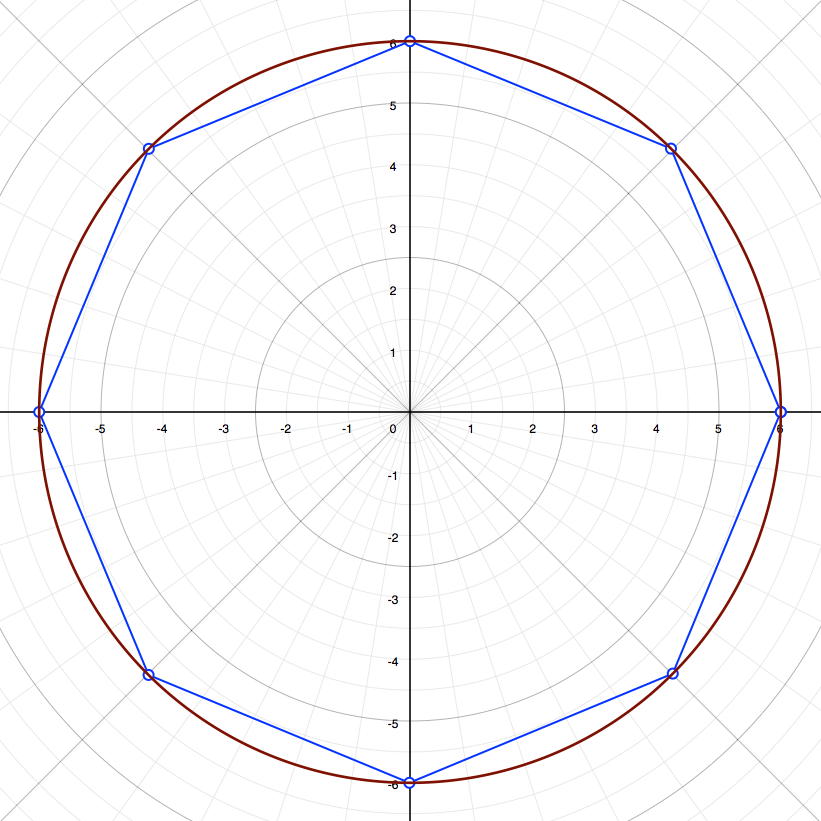
\includegraphics[width=3in]{g10a.png}





\newpage
10. Sketch each curve with the given polar equation. \\
\\
\indent (b) $r=\frac{1}{2}\theta,\ -4\pi \leq \theta \leq 4\pi$\\
\newline
\newline
\def\arraystretch{1.5}
\begin{tabular}{ c|c }
  $\theta$ & $r$ \\
  \hline
  0                & 0                \\
  $\frac{\pi}{4}$  & $\frac{\pi}{8}$  \\
  $\frac{\pi}{2}$  & $\frac{\pi}{4}$  \\
  $\frac{3\pi}{4}$ & $\frac{3\pi}{8}$ \\
  $\pi$            & $\frac{\pi}{2}$  \\
  $\frac{5\pi}{4}$ & $\frac{5\pi}{8}$ \\
  $\frac{3\pi}{2}$ & $\frac{3\pi}{4}$ \\
  $\frac{7\pi}{4}$ & $\frac{7\pi}{8}$ \\
  $2\pi$           & $\pi$            \\
\end{tabular}\\
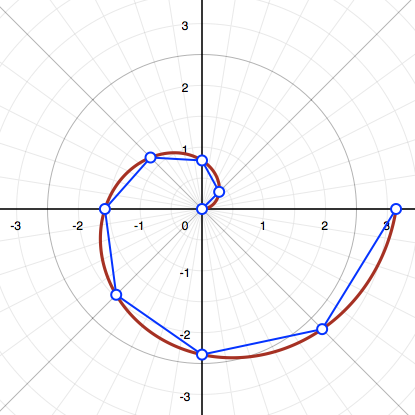
\includegraphics[width=3in]{g10b.png}





\newpage
10. Sketch each curve with the given polar equation. \\
\\
\indent (c) $\theta=\frac{\pi}{6}$\\
\newline
\newline
\def\arraystretch{1.5}
\begin{tabular}{ c|c }
  $\theta$ & $r$ \\
  \hline
  $\frac{\pi}{6}$ & -10 \\
  $\frac{\pi}{6}$ & -5  \\
  $\frac{\pi}{6}$ &  0  \\
  $\frac{\pi}{6}$ &  5  \\
  $\frac{\pi}{6}$ &  10 \\
\end{tabular}\\
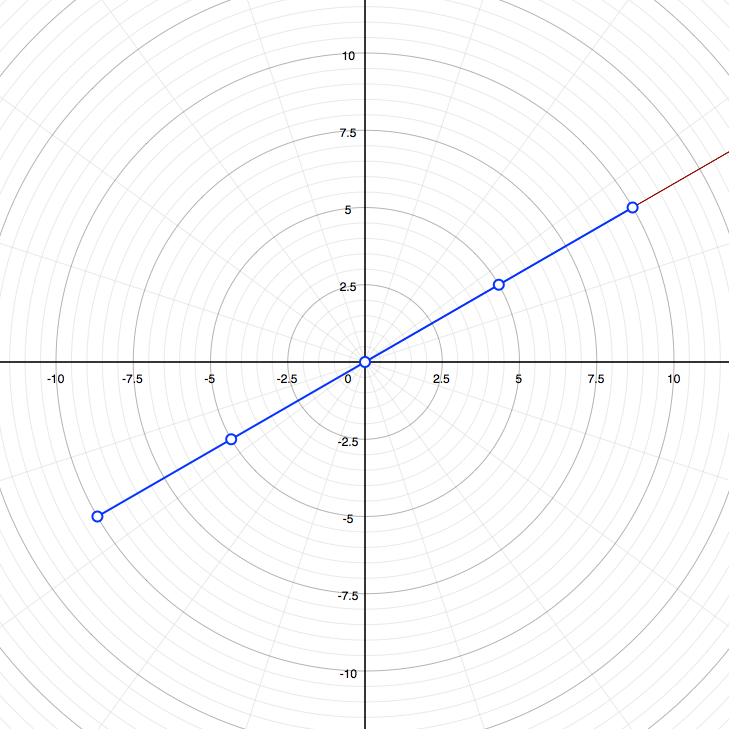
\includegraphics[width=3in]{g10c.png}





\newpage
10. Sketch each curve with the given polar equation. \\
\\
\indent (d) $r=1+ \cos \theta$\\
\newline
\newline
\def\arraystretch{1.5}
\begin{tabular}{ c|c }
  $\theta$ & $r$ \\
  \hline
  0                & 2    \\
  $\frac{\pi}{4}$  & 1.71 \\
  $\frac{\pi}{2}$  & 1    \\
  $\frac{3\pi}{4}$ & 0.29 \\
  $\pi$            & 0    \\
  $\frac{5\pi}{4}$ & 0.29 \\
  $\frac{3\pi}{2}$ & 1    \\
  $\frac{7\pi}{4}$ & 1.71 \\
  $2\pi$           & 2    \\
\end{tabular}\\
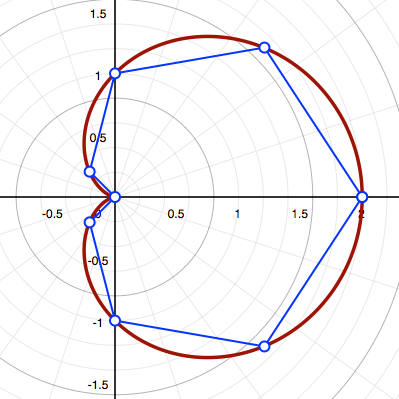
\includegraphics[width=3in]{g10d.png}




\end{document}